
\section{Grammars For Formal Languages}

A Grammar or A formal Grammar is a set of rules for writing strings in a formal language, along with a "start symbol" from which rewriting must start.Therefore, a grammar is usually thought of as a language generator. The rules tell how to form strings from the language's letters that are valid according to the language's syntax. A grammar does not describe the meaning of the strings rather  what can be done with them in their rightful context form.\\


Formal language theory,is a branch of applied mathematics which studies formal grammars and languages. Its applications are found many areas such as mathematical logic, theoretical computer science, theoretical linguistics, formal semantics,  and other areas.\\


parsing a string of characters is analyzing this string to find tokens, or items and then create a structure from the result.


akjhf  dkfh  lskdfh 


\subsection{Vocabulary}

We need to review some basic  definitional terms.
\begin{enumerate}
\item [grammar :] a set of rules by which valid sentences in a language are constructed.\\

a set of rules which constructed a correct sentences in a language .\\

\item [nonterminal symbols:] are those grammar symbols which can be replaced/expanded to a sequence of symbols.They may also be called simply syntactic variables\\



\item [terminal symbols:]  are literal symbols which may appear in the outputs of the production rules of a formal grammar and which cannot be changed using the rules of the grammar..\\

\item [production :] a grammar rule that describes how to replace/exchange symbols. The general form of a production for a nonterminal is:\\



X –$>$Y 1 Y 2 Y 3 ...Y n\\

The nonterminal X is declared equivalent to the concatenation of the symbols Y 1 Y 2 Y 3 ...Y n . The production means that anywhere where we encounter X , we may replace it by the string Y 1 Y 2 Y 3 ...Y n . Eventually we will have a string containing nothing that can be expanded further, i.e., it will consist of only terminals. Such a string is called a sentence. In the context of programming languages, a sentence is a syntactically correct and complete program.\\

\item [derivation :] a sequence of applications of the rules of a grammar that produces a finished string of terminals. A leftmost derivation is where we always substitute for the leftmost nonterminal as we apply the rules (we can similarly define a rightmost derivation). A derivation is also called a parse.\\

\item [start symbol :] a grammar has a single nonterminal (the start symbol) from which all sentences derive:\\

S –$>$ X 1 X 2 X 3 ...X n\\

All sentences are derived from S by successive replacement using the productions of the grammar.\\

\item [null symbol $\epsilon$ :] it is sometimes useful to specify that a symbol can be replaced by nothing at all. To indicate this, we use the null symbol $\epsilon$, e.g., A –$>$ B | $\epsilon$.\\

\item [BNF :] a way of specifying programming languages using formal grammars and production rules with a particular form of notation (Backus-Naur form).\\

\end{enumerate}



\subsection{A Hierarchy of Grammars}

Grammars can be divided into four classes by gradually increasing the restrictions on the form of
the productions. Such a classification is due to Chomsky [Chomsky, 1956, Chomsky, 1963] and is called the Chomsky hierarchy.
\\
this four categories of formal grammars in the Chomsky Hierarchy, they span from Type 0, the most general, to Type 3, the most restrictive. More restrictions on the grammar make it easier to describe and efficiently parse, but reduce the expressive power.\\


Type 0: free or unrestricted grammars\\
These are the most general. Productions are of the form u –$>$ v where both u and v are arbitrary strings of symbols in V, with u nonnull. There are no restrictions on what appears on the left or righthand side other than the left-hand side must be non-empty.\\


Type 1: context-sensitive grammars\\
Productions are of the form uXw –$>$ uvw where u , v and w are arbitrary strings of symbols in V, with v non-null, and X a single nonterminal. In other words, X may be replaced by v but only when it is surrounded by u and w . (i.e., in a particular context).\\

Type 2: context-free grammars\\
Productions are of the form X–$>$ v where v is an arbitrary string of symbols in V,and X is a single nonterminal. Wherever you find X, you can replace with v (regardless of context).\\

Type 3: regular grammars\\
Productions are of the form X–$>$ a, X–$>$ aY, or X–$>$ $\epsilon$  where X and Y are nonterminals and a is a terminal. That is, the left-hand side must be a single nonterminal and the right-hand side can be either empty, a single terminal by itself or with a single nonterminal. These grammars are the most limited in terms of expressive power.\\

Every type 3 grammar is a type 2 grammar, and every type 2 is a type 1 and so on. Type 3 grammars are particularly easy to parse because of the lack of recursive constructs.
Efficient parsers exist for many classes of Type 2 grammars. Although Type 1 and Type 0
grammars are more powerful than Type 2 and 3, they are far less useful since we cannot
create efficient parsers for them. In designing programming languages using formal
grammars, we will use Type 2 or context-free grammars, often just abbreviated as CFG.



\subsection{Parsing Issues}


There are several issues that can interfere with parsing that we must take into consideration when designing the grammar.Let’s take a look at three of them: ambiguity, recursive rules, and left-factoring.

\begin{enumerate}
\item Ambiguity:

A grammar is ambiguous if some phrase in the language generated by the grammar has two distinct derivation trees. For instance, the grammar below, which we have been using as our running example, is ambiguous.



For example, consider the expression 8 + 2 * 3 which indicates that this grammar is ambiguous we can observe that it is possible to derive two different syntax trees for this expression.
We parse by first applying the production E –> E op E.The parse tree on the left chooses to expand that first op to *, the one on the right to +. We have two completely different parse trees,the figure below shows these two different derivation trees:\\





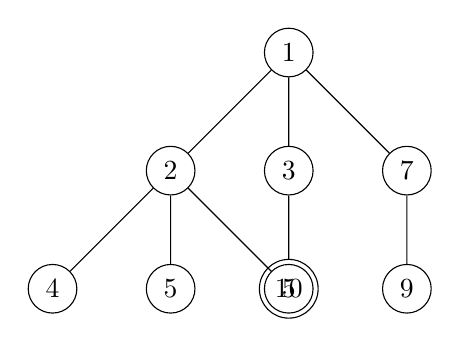
\begin{tikzpicture}[every node/.style={circle,draw=black,sibling distance = 5cm,level distance = 4.5cm}]
\node{1}
  child{node{2}
  child{node{4}}
  child{node{5}}  
  child{node{5}}   
  }child{node{3}
  child{node{10}}
     }
     child{node{7}
child{node{9}}     
     }
     ;
\end{tikzpicture}



\item Recursive productions :
Productions are often defined in terms of themselves. For example a list of variables in a programming language grammar could be specified by this production:

\item left-factoring:  A parser usually reads tokens from left to right and it is convenient if, upon reading a token, it can make an immediate decision about which production from the grammar to expand. However, this can be trouble if there are productions that have common prefix. Here is an example we often see in programming language grammars:\\










Stmt–$>$if Cond then Stmt else Stmt|if Cond then Stmt | Other|...\\


1) we can see that , for every production , there is a common prefix (if Cond then Stmt) if we choose any production here , it is not cofirmed that we will not need to backtrack.
2) it is non deterministic , because we cannot choice any production and be assured that we will reach at our desired string by making the correct parse tree. but if we rewrite the grammar in a way that is deterministic and also leaves us to be flexible enough to make it any string that may be possible without backtracking .... it will be : 






Stmt –$>$ if Condition then Stmt OptElse | Other | ...\\
OptElse –$>$ else S | $\epsilon$ \\
In the re-written grammar, upon reading an “if” we expand first production and wait until if Cond then Stmt has been seen to decide whether to expand OptElse to else or $\epsilon$.



\end{enumerate}




\subsection{Parsing Techniques}
Parsing a sentence means to compute the structural description (descriptions) of the sentence assigned by a grammar, assuming, of course, that the sentence is well-formed. Mathematical work on parsing consists of at least the following activities.\\

\begin{enumerate}
\item Mathematical characterization of derivations in a grammar and the associated parsing algorithms. 

\item Computing the time and space complexities of these algorithms in terms of the length of the sentence and the size of the grammar, primarily,

\item Comparing different grammar formalisms and showing equivalences among them wherever possible, thereby developing uniform parsing algorithms for a class of grammars.

\item Characterizing parsing as deduction and a uniform specification of parsing algorithms for a wide class of grammars.


\item Combining grammatical and statistical information for improving the efficiency of parsers and ranking of multiple parses for a sentence.

\end{enumerate}

The structural descriptions provided by a grammar depend on the grammar formalism to which the grammar belongs. For the well-known context-free grammar (CFG) the structural description is, of course, the conventional phrase structure tree (tress) associated with the sentence. The parse tree describes the structure of the sentence. It is also the record of the history of derivation of the sentence. Thus, in this case the structural description and the history of the derivation are the same objects. Later, we will comment on other grammar formalisms and the structural descriptions and histories of derivation associated with them. 





\section{Triangular Expressions}
We will speak in general and describe what is Section do,then we will give some example if it is necessary

\section{Mobile Application}
We will speak in general and describe what is Section do,then we will give some example if it is necessary

\subsection{Android}
We will speak in general and describe what is Section do,then we will give some example if it is necessary



\section{Security}
We will speak in general and describe what is Section do,then we will give some example if it is necessary

\subsection{Introduction}
We will speak in general and describe what is Section do,then we will give some example if it is necessary

\subsection{QRCode}
QR is short for Quick Response, which is given because
a cell phone can read the code quickly. QR codes are used
to take a piece of information from a transitory media and
put it into your cell phone.

\subsection{Encryption and Decryption}
Encryption provides the ability to use mathematical
algorithms to protect the confidentiality and integrity of
information transmitted via insecure means or stored in an
insecure location. While the detailed mathematics underlying
encryption may be intimidating, the basic concepts are quite
accessible, and all technology professionals should have at
least a basic understanding of how encryption provides these
security benefits.
Encryption takes cleartext data and uses a mathematical
algorithm, in conjunction with an encryption key, to convert
it into a form that is only readable by someone who knows
the algorithm that was used and has access to the proper
decryption key. This encrypted data is often referred to
as the ciphertext. The encryption algorithm may be from
one of two classes: symmetric algorithms and asymmetric
algorithms.



\section{Language Interpreters}

\subsection{Lexical Analysis (regular expressions)}


Lexical analysis is the extraction of individual words or lexemes from an input stream of symbols and passing corresponding tokens back to the parser.\\

If we consider a statement in a programming language, we need to be able to recognise the small syntactic units (tokens) and pass this information to the parser. We need to also store the various attributes in the symbol or literal tables for later use, e.g., if we have an variable, the tokeniser would generate the token var and then associate the name of the variable with it in the symbol table - in this case, the variable name is the lexeme.\\

Other roles of the lexical analyser include the removal of whitespace and comments and handling compiler directives (i.e., as a preprocessor).\\

The tokenisation process takes input and then passes this input through a keyword recogniser, an identifier recogniser, a numeric constant recogniser and a string constant recogniser, each being put in to their own output based on disambiguating rules.\\

These rules may include "reserved words", which can not be used as identifiers (common examples include begin, end, void, etc), thus if a string can be either a keyword or an identifier, it is taken to be a keyword. Another common rule is that of maximal munch, where if a string can be interpreted as a single token or a sequence of tokens, the former interpretation is generally assumed.\\


The lexical analysis process starts with a definition of what it means to be a token in the language with regular expressions or grammars, then this is translated to an abstract computational model for recognising tokens (a non-deterministic finite state automaton), which is then translated to an implementable model for recognising the defined tokens (a deterministic finite state automaton) to which optimisations can be made (a minimised DFA).




\subsection{Syntax Analysis }

Syntactic analysis, or parsing, is needed to determine if the series of tokens given are appropriate in a language - that is, whether or not the sentence has the right shape/form. However, not all syntactically valid sentences are meaningful, further semantic analysis has to be applied for this. For syntactic analysis, context-free grammars and the associated parsing techniques are powerful enough to be used - this overall process is called parsing.\\

In syntactic analysis, parse trees are used to show the structure of the sentence, but they often contain redundant information due to implicit definitions (e.g., an assignment always has an assignment operator in it, so we can imply that), so syntax trees, which are compact representations are used instead. Trees are recursive structures, which complement CFGs nicely, as these are also recursive (unlike regular expressions).\\

There are many techniques for parsing algorithms (vs FSA-centred lexical analysis), and the two main classes of algorithm are top-down and bottom-up parsing.\\

Context-free grammars can be represented using Backus-Naur Form (BNF). BNF uses three classes of symbols: non-terminal symbols (phrases) enclosed by brackets <>, terminal symbols (tokens) that stand for themselves, and the metasymbol ::= - is defined to be.\\

As derivations are ambiguous, a more abstract structure is needed. Parse trees generalise derivations and provide structural information needed by the later stages of compilation.

\subsubsection{BNF} 

Backus-Naur notation (more commonly known as BNF or Backus-Naur Form) is a formal mathematical way to describe a language, which was developed by John Backus (and possibly Peter Naur as well) to describe the syntax of the Algol 60 programming language.

(Legend has it that it was primarily developed by John Backus (based on earlier work by the mathematician Emil Post), but adopted and slightly improved by Peter Naur for Algol 60, which made it well-known. Because of this Naur calls BNF Backus Normal Form, while everyone else calls it Backus-Naur Form.)

It is used to formally define the grammar of a language, so that there is no disagreement or ambiguity as to what is allowed and what is not. In fact, BNF is so unambiguous that there is a lot of mathematical theory around these kinds of grammars, and one can actually mechanically construct a parser for a language given a BNF grammar for it. (There are some kinds of grammars for which this isn't possible, but they can usually be transformed manually into ones that can be used.)

Programs that do this are commonly called "compiler compilers". The most famous of these is YACC, but there are many more.



\subsubsection{EBNF}

In DL I had to use recursion (ie: DL can produce new DLs) to express the fact that there can be any number of Ds. This is a bit awkward and makes the BNF harder to read. Extended BNF (EBNF, of course) solves this problem by adding three operators:\\

    ? : which means that the symbol (or group of symbols in parenthesis) to the left of the operator is optional (it can appear zero or one times)
    * : which means that something can be repeated any number of times (and possibly be skipped altogether)
    + : which means that something can appear one or more times



\subsubsection{syntax classes}

\subsubsection{AST}


\subsection{Semantics Analysis}
Semantic analysis is needed to check aspects that are not related to the syntactic form, or that are not easily determined during parsing, e.g., type correctness of expressions and declaration prior to use.
\subsection{Evaluation Methods}

\subsubsection{instanceof}

\subsubsection{ eval()}

\subsubsection{visitor}



\section{Automatic Code Generation Tools}
We will speak in general and describe what is Section do,then we will give some example if it is necessary

\subsection{javacc}
JavaCC is a parser generator and a lexical analyzer generator. Parsers and lexical analysers
are software components for dealing with input of character sequences. Compilers and
interpreters incorporate lexical analysers and parsers to decipher files containing programs,
however lexical analysers and parsers can be used in a wide variety of other applications,
as I hope the examples in this boo kwill illustrate.
So what are lexical analysers and parsers? Lexical analysers can brea ka sequence of
characters into a subsequences called
tokens
and it also classifies the tokens. Consider a
short program in the C programming language.

\subsection{Yacc}
We will speak in general and describe what is Section do,then we will give some example if it is necessary


\subsection{Android Sudio}
We will speak in general and describe what is Section do,then we will give some example if it is necessary

\subsection{Latex}
We will speak in general and describe what is Section do,then we will give some example if it is necessary

